
\chapter{Cross-validation for unsupervised learning}


\begin{figure}[tbh]
    \centering
    \begin{minipage}{0.38\textwidth}
        \begin{center}
            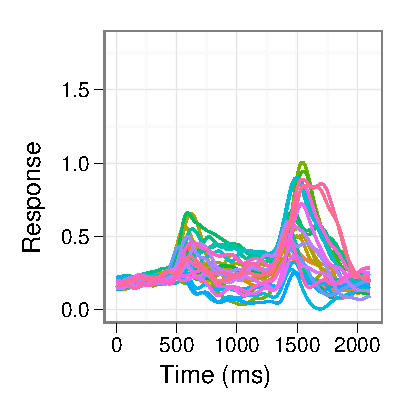
\includegraphics{neuron1}
        \end{center}
    \end{minipage}
    \begin{minipage}{0.61\textwidth}
        \begin{center}
            \includegraphics{neurons}
        \end{center}
    \end{minipage}
    \caption{
        \captiontitle{Motor Cortex Data}
        Response rates in 47 neurons for 27 movement tasks.  The subplots show
        the normalized response rates in a single neuron as functions of time.  
        Each color corresponds to a different movement task.  The plot on
        the left is a zoomed-in view of the data for the first neuron.
    }
\end{figure}
